TODO: watch out for $c=1$.

\chapter{Gravity and covariance}
In the previous section we have discussed relativistic mechanics and rewritten the laws of electrodynamics in a covariant way. Now we turn to gravity; the goal of general relativity is to find a relativistic theory of gravity.

Electrodynamics was already intrinsically relativistic. Unfortunately we are not so lucky with Newton's theory of gravity. It has some decidedly non-relativistic properties that mean that it must be an approximation of a more fundamental theory.

We can express Newton's theory of gravity as follows (see also the section on Newtonian mechanics):
\[ \vec{F}_{12} = -G_N \frac{m_1m_2}{|\vec{r}_1 - \vec{r}_2|^2} \hat{n}_{12} \qquad \left(\hat{n}_{12} \; \text{is the unit vector} \; \frac{\vec{r}_1 - \vec{r}_2}{|\vec{r}_1 - \vec{r}_2|}\right) \]

Problems for making it covariant include:
\begin{itemize}
\item Gravity depends on a \ueig{spatial distance} measured at a \ueig{given time}, both of which are not invariant. According to which observer should we measure these quantities?
\item There is an \ueig{action at a distance}: Newtonian gravity acts instantly. However no signal can move faster than the speed of light. This is a problem. 
\end{itemize}

Of course it is not always necessary to use \emph{relativistic} gravity. Newtonian gravity is adequate in many situations. In particular the Newtonian approximation is a good one if
\[ \frac{G_NM}{Rc^2} \]
is much less than one. Otherwise we must use the formulae for relativistic gravity.

\chapter{Equivalence principles}
\section{Weak equivalence principle}
\[ \vec{F}_g = -m_g \vec{\nabla}\Phi \qquad \vec{a}= \frac{\vec{F}_g}{m_I} = -\left(\frac{m_g}{m_I}\right)\vec{\nabla}\Phi \]
The weak equivalence principle states that
\[ m_g = m_I \]
Which means that the acceleration of an object due to gravity is independent of the nature of the object. In other words gravity is purely geometric.

Equivalently we can state the WEP as follows
\begin{eigenschap}
The motion of freely-falling particles are the same in a gravitational field and a uniformly accelerated frame, in small enough regions of space.
\end{eigenschap}

\section{Einstein equivalence principle}
The basic idea is that locally there is no way to distinguish between uniform acceleration and an external gravitational field, no matter what the experiment (so it applies to all of physics). Formally
\begin{eigenschap}
In small enough regions of spacetime, the laws of physics reduce to those of spacial relativity; it is impossible to detect the existence of a gravitational field by means of local experiments.
\end{eigenschap}
\begin{enumerate}
\item The weak equivalence principle holds
\item There is local Lorentz invariance (the space is locally Minkowski and special relativity holds)
\remark{It is impossible to detect gravity through local, non-gravitational experiments}
\item There is local position invariance.
\[ \partial_\mu g_{\nu\rho}(x_p) = 0 \]
\end{enumerate}
Local Lorentz invariance has been verified to $10^{-24}$ and local position invariance to $10^{-4}$.

We can tell acceleration from gravity if time / space is long enough:

\begin{tikzpicture}
\draw (0,0) -- (4,0) -- (4,1.5) -- (0,1.5) -- cycle; 
\pic[draw, very thick, scale=.25] at (.5,1) {apple};
\pic[draw, very thick, scale=.25] at (3.5,1) {apple};
\draw[->] (.8, 0.5) -- (1.025,.125);
\draw[->] (3.2, 0.5) -- (2.975,.125);
\draw (2,-1.1) circle (1);
\end{tikzpicture}

In general iff no nonuniformities of $\Phi$ can be detected.

\section{Strong equivalence principle}
Object only feels result of curvature from \undline{other objects}.
\remark{self-interaction strongly limited}
\begin{eigenschap}
General relativity is uniquely compatible with the strong equivalence principle.
\end{eigenschap}

\section{Experimental evidence}
\subsection{Eötvös experiment}
[Insert picture here]
Eötvös parameter:
\[ \eta = 2 \frac{a_2-a_1}{a_2+a_1} = \frac{\left(\frac{m_g}{m_I}\right)_2 - \left(\frac{m_g}{m_I}\right)_1}{\left(\frac{m_g}{m_I}\right)_2 + \left(\frac{m_g}{m_I}\right)_1} \]
With the following results:
\begin{align*}
\eta_{\text{Be},\text{T}} &= (0,3 \pm 1,8)\cdot 10^{-13} \\
\eta_{\text{Be},\text{Al}} &= (-0,7 \pm 1,3)\cdot 10^{-13} \\
\eta_{\text{Earth},\text{Moon}} &= (\quad \pm \quad)\cdot 10^{} \\
\end{align*}

\subsection{MICROSCOPE}
MICRO-Satellite à traînée Compensée pour l'Observation du Principe d'Equivalence (MICROSCOPE). Tests WEP up to $10^{-15}$.
\[ \eta < 2,1\times 10^{-14} \]

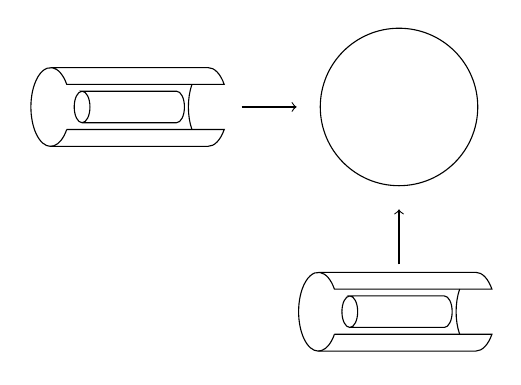
\begin{tikzpicture}[microscope/.pic={
\path (0,0) -- ++(-1.55,0) arc (0:360-35:.5 and 1) coordinate (start);
\path (start)  arc (360-35:90:.5 and 1) coordinate (p1);
\path (start)  arc (360-35:270:.5 and 1) coordinate (p2);
\draw (start) arc (360-35:35:.5 and 1) -- ++(4,0) arc (35:90:.5 and 1) -- (p1);
\draw (start) -- ++(4,0) arc (360-35:360-90:.5 and 1) -- (p2);
\path (start) -- ++(4,0)  arc (360-35:180+35:.5 and 1) coordinate (p3);
\draw (p3) arc (180+35:180-35:.5 and 1);
\path (start) arc (360-35:0:.5 and 1) -- ++ (.5,0) arc (0:90:.2 and .4) coordinate (c2);
\draw (c2) arc (90:360+90:.2 and .4) -- ++(2.4,0) arc (90:90-180:.2 and .4) -- ++(-2.4,0);
}]
\pic[draw, scale=.5] at (-3.4,0) {microscope};
\pic[draw, scale=.5] at (0,-2.6) {microscope};
\draw[->] (-2,0) -- (-1.3,0);
\draw[->] (0,-2) -- (0,-1.3);
\draw (0,0) circle (1);
\end{tikzpicture}

\section{Towards general covariance}
\subsection{Newtonian gravity in spacetime terms}
6.6 Hartle
\[ \diff{s}^2 = - \left(1+ \frac{2\Phi(x^i)}{c^2}\right)(c \diff{t})^2 + \left(1- \frac{2\Phi(x^i)}{c^2}\right)(\diff{x}^2 + \diff{y}^2 + \diff{z}^2) \]
Static weak field approximation


\chapter{Consequences of the equivalence principles and overview of general relativity}
In this section we explore some of the consequences of the equivalence principles. Then we give a very quick overview of way we will be building up the theory of general relativity in this section. This should hopefully serve to justify the somewhat involved mathematics of the next section.

\section{Gravitational redshift}
\[ \omega_\infty = \left(1- \frac{G_N M}{Rc^2}\right)\omega_* \]

\section{Geometric interpretation of gravity}
spacetime: differentiable manifold
Chapt 6.5 Hartle

Gravity as a property of space, so we need to review how we see space. We need it to be approximately flat in small areas. This idea is captured in the rigourous, mathematical notion of a manifold.

We take spacetime to be a differentiable manifold, meaning we can still do calculus to points in the manifold.

We also still want to be able to use vectors, and in general tensors, on the manifold. Here we run into a slight problem: vectors in different points are incompatible with each other. Concepts such as the displacement and position vector only work in flat space. Instead we construct a vector space (and more generally tensors) in each point. That vector space is called the tangent space in a point. (TODO Why + link to curvature)

We can however link the tangent spaces in neighbouring points using connections. These are not inherent in a manifold and specify the curvature. There is another (more intuitive) way to specify the curvature: using a metric. Here our concept of metric will be slightly different (!) than when we discussed metric spaces above. A major difference will be that we will not require it to be positive definite.

\section{Causality}



\section{Rindler spacetime}
\subsection{Uniformly accelerated observers}
\[ \diff{s}^2 = - \diff{t}^2 + \diff{x}^2 \]
We study uniformly accelerating object (indestiguishable from gravity in local experiments):
\[ \alpha^2 = \alpha^\mu\alpha_\mu = a^2 \qquad x(0) = \frac{1}{a} \]
With $\alpha$ the acceleration.
Following is basic SR kinematics
\[x(t) = x(0) + \frac{1}{a} \sqrt{1+a^2t^2}- \frac{1}{a} = \frac{1}{a} \sqrt{1+a^2t^2}\]
\[ \begin{cases}
t(\tau) = \frac{1}{a} \sinh(a\tau) \\
x(\tau) = \frac{1}{a} \sqrt{1+\sinh^2(a\tau)}
\end{cases} \qquad x^\mu(\tau) = \frac{1}{a} \begin{pmatrix}
\sinh(a\tau) \\ \cosh(a\tau)
\end{pmatrix}\]

%See drawing
[Note to self: look up Minkowski diagram]

Still compatible with assumptions:
\[ u^\mu = \od{x^\mu}{\tau} = \begin{pmatrix}
\cosh(a\tau) \\ \sinh(a\tau)
\end{pmatrix} \qquad \alpha^\mu \od[2]{x^\mu}{\tau} = a \begin{pmatrix}
\sinh(a\tau) \\ \cosh(a\tau)
\end{pmatrix} \]
\[\alpha^\mu\alpha_\mu = a^2 (-\sinh^2(a\tau)+\cosh^2(a\tau)) = a^2\]

\subsection{Adapted coordinates}
Change variables so that $\xi = 0$ gives trajectory of object.
\[ \begin{pmatrix}
t \\ x
\end{pmatrix} \mapsto \begin{pmatrix}
\tau \\ \xi
\end{pmatrix} \]
A t = 0 both observers have same spacetime

Change of coordinates is singular: can only describe part of spacetime.

\[ \begin{cases}
t (\tau, \xi = 0) = \frac{1}{a} \sinh(a\tau) \\
x(\tau, \xi = 0) = \frac{1}{a} \cosh(a\tau)
\end{cases}\]
\[ x(\tau = 0, \xi) = \frac{f(\xi)}{a} ?? \]

We want $x = 0$ is $\xi = -\infty$, so $\log$, because $x=0$ will be singular:
\[ x \in ]0,+\infty[, t \in \R \to \xi \in \R, \tau \in \R \]
So we choose:
\[ \begin{cases}
t (\tau, \xi) = \frac{e^{a\xi}}{a} \sinh(a\tau) \\
x(\tau, \xi) = \frac{ e^{a\xi} }{a} \cosh(a\tau)
\end{cases}\]
\[ \begin{cases}
\tau(t,x) = \frac{1}{a} \atanh(t/x) \\
\xi(t,x) = \frac{1}{2a} \log[a^2(x^2 - t^2)]
\end{cases} \]
Argument of $\log$ has to be positive, so only describes wedge, not even light cone.

\[ \diff{s}^2 = - \diff{t}^2 + \diff{x}^2 \]
\begin{align*} \diff{s}^2 &= -\left(\pd{t}{\xi} \diff{\xi} + \pd{t}{\tau} \diff{\tau}\right)^2+\left( \pd{x}{\xi} \diff{\xi} + \pd{x}{\tau} \diff{\tau} \right)^2 \\
=& -(e^{a\xi}\sinh(a\tau)\diff{\xi} + e^{a\xi}\cosh(a\tau)\diff{\tau})^2
+(e^{a\xi}\cosh(a\tau)\diff{\xi} + e^{a\xi}\sinh(a\tau)\diff{\tau})^2
=& e^{2a\xi}
\end{align*}

\[ \diff{s}^2 = - \diff{t}^2 + \diff{x}^2 = e^{2a\xi}(- \diff{\tau}^2 + \diff{\xi}^2)\]

\subsection{Rindler spacetime (time dilation, event horizons)}

Now take observer at $\xi = 0$, so $t = \frac{1}{a}\sinh(a\tau)$ and $x = \frac{1}{a} \cosh(a\tau)$. Then observe $\xi = 1$:
\[ \begin{cases}
t = \frac{e^{a}}{a} \sinh(a\tau) = \frac{1}{a'} \sinh(a'\tau') \qquad a'=ae^{-a} < a\\
x = \frac{e^{a}}{a} \cosh(a\tau) = \frac{1}{a'} \cosh(a'\tau') \qquad \tau' = \frac{a}{a'} \tau = e^{a}\tau > \tau
\end{cases} \]
Less acceleration means time flows faster, more acceleration means time flows slower.

Now for $\xi = -1$:
\[ \begin{cases}
t = \frac{e^{-a}}{a} \sinh(a\tau) = \frac{1}{a''} \sinh(a''\tau'') \qquad a''=ae^{a} > a\\
x = \frac{e^{-a}}{a} \cosh(a\tau) = \frac{1}{a''} \cosh(a''\tau'') \qquad \tau'' = \frac{a}{a''} \tau = e^{-a}\tau < \tau
\end{cases} \]

Clock in satellite: two competing effects.

Redshift: $\sqrt{-g_{\tau\tau}} = \sqrt{e^{2a\xi}} = e^{a\xi}$


Even if metric is singular, the space is not singular! (Extend I to II, and then to IV)

\[ g_{\mu\nu} = \begin{pmatrix}
-e^{2a\xi} & 0 \\
0& e^{2a\xi}
\end{pmatrix} \qquad \partial_{\tau}g_{\mu\nu} = 0 \]

\[u^{\mu} = \begin{pmatrix}
1\\ 0
\end{pmatrix} \qquad u = \partial_\tau\]

\begin{align*}
u^\mu u_\mu &= g_{\tau\tau} = -e^{2a\xi} < 0 \\
&= a^2(t^2-x^2)
\end{align*}
$u$ is timelike in I as it should be, but can also be lightlike or spacelike in different sections.





\chapter{Explaining the geometry of gravity: Einstein's equations}
\section{The Einstein-Hilbert action}
\section{Einstein's equations}
\section{The stress-energy tensor}
(stress tensor for a gas of particles)

\section{Couplings to other fields}

\[x^\mu : \R \to \R^{1,3}: \tau \mapsto \]

% See notes

Now we describe free motion of massive particle. The action is:
\[ S[x^\mu(\tau)] = -m\int \diff{s} \]
Describe for arbitrary metric
\[\diff{s}^2 = \diff{x}^\mu \diff{x}^\nu g_{\mu\nu}(x)\]
Extremise $S$! Trajectory of massive particle given by maximum. (Massless more difficult).
\[\delta S = -m\int \delta\left(\sqrt{-\dot{x}^\mu\dot{x}^\nu g_{\mu\nu}(x)}\right)\diff{\tau} = m \int \frac{1}{2\sqrt{-\dot{x}^2}}\left(2\dot{x}^\mu \od{\delta x^\nu}{\tau} g_{\mu\nu} + \dot{x}^\mu\dot{x}^\nu \pd{g_{\mu\nu}}{x^\rho}\delta x^\rho\right) \diff{\tau}\]
Using that $\dot{x}^2$ is constant, this is equal to
\[ m\int \frac{1}{2\sqrt{-\dot{x}^2}}\left(\ddot{x}^\mu g_{\mu\nu} \delta x^\nu - \dot{x}^\mu \delta x^\nu \pd{g_{\mu\nu}}{x^\rho}\dot{x}^\rho + \frac{1}{2} \dot{x}^\mu \dot{x}^\nu \pd{g_{\mu\nu}}{x^\rho} \delta x^\rho\right) \diff{\tau} = 0\]
\begin{align*} \delta S &= -m \int \frac{1}{2\sqrt{-\dot{x}^2}}\left(\ddot{x}^\mu g_{\mu\rho} + \dot{x}^\mu \dot{x}^\nu \partial_\nu g_{\mu\rho} - \frac{1}{2} \dot{x}^\mu \dot{x}^\nu \partial_\rho g_{\mu\rho}\right)\delta x^\rho \diff{\tau} \\
&= -m \int \frac{g_{\mu\rho}}{2\sqrt{-\dot{x}^2}}\left(\ddot{x}^\mu + g^{\mu\sigma} \partial_\tau g_{\mu\rho} \dot{x}^\nu \dot{x}^\tau - \frac{1}{2}g^{\mu\sigma}\partial_\sigma g_{\mu\tau}\dot{x}^\nu \dot{x}^\tau\right)\delta x^\rho \diff{\tau}
\end{align*}

\[ \delta S = -m \int \frac{g_{\mu\rho}}{2\sqrt{-\dot{x}^2}} \frac{D\dot{x}^\mu}{D\tau} \delta x^\rho \diff{\tau}\]
\[ \frac{D\dot{x}^\mu}{D\tau} =  \od[2]{x^\mu}{\tau} + \frac{1}{2} g^{\mu\sigma} \left(\partial_\nu g_{\rho\sigma} + \partial_\rho g_{\nu\sigma} - \partial_\sigma g_{\nu\rho}\right)\dot{x}^{\nu}\dot{x}^\rho = 0\]
Christoffel symbols
\[ \Gamma^\mu_{\nu\rho} \equiv \frac{1}{2} g^{\mu\sigma} \left(\partial_\nu g_{\rho\sigma} + \partial_\rho g_{\nu\sigma} - \partial_\sigma g_{\nu\rho}\right)\]
What about partical with other parameter than $\tau$? Or massless particles?
We want a procedure that is reparametrisation invariant.
Change of coordinates that is never singular:
\[ \tau \to \tau'= \tau'(\tau) \qquad \od{\tau'}{\tau} \neq 0 \qquad \diff{s}^2 = \diff{x}^\mu \diff{x}^\nu g_{\mu\nu}(x)\]
\[ \diff{s}^2 = \diff{\tau}^2\gamma_{\tau\tau}(\tau) = \diff{\tau'}\diff{\tau'}\gamma_{\tau'\tau'} = \diff{\tau'}\diff{\tau'}\od{\tau}{\tau'}\od{\tau}{\tau'}\gamma_{\tau\tau}\]
\[ \gamma_{\tau'\tau'} = \left(\od{\tau}{\tau'} \right)^2\gamma_{\tau\tau} \]
\[ \gamma_{\tau\tau} = \left(\od{\tau}{\tau'} \right)^2\gamma_{\tau'\tau'} \]
Proper time: $\gamma_{\tau\tau} = -1$
Polyakov's action:
\[ S = - \frac{1}{2} \diff{\tau} \sqrt{\gamma} \left[ \gamma^{\tau\tau} \od{x^\mu}{\tau} \od{x^\nu}{\tau} g_{\mu\nu}(x) + m^2 \right] \]
($\tau$ generic parameter)

We can also describe motion of particle, string or brane:
\begin{itemize}
\item 0-dim object $\to$ 1-dim worldline
\item 1-dim object $\to$ 2-dim worldsheet
\end{itemize}

Write action in terms of $e$ ($\gamma_{\tau\tau}(\tau) = -e^2(\tau)$)
\[ S[x^\mu,e] = \frac{1}{2} \int \diff{\tau} [e^{-1}\dot{x}^\mu\dot{x}^\nu g_{\mu\nu} - em^2] \]
\begin{align*} \frac{\delta S}{\partial x^\mu} &\sim e^{-1}[2\dot{x}^\mu \delta \dot{x}^\nu g_{\mu\nu} + \dot{x}^\mu\dot{x}^\nu \partial_\rho g_{\mu\nu} \delta x^\rho] \\ &= \int \diff{\tau}e^{-1} \left[ - \frac{D\dot{x}^\mu}{D\tau} g_{\mu\nu} \delta x^\nu \right] = 0 \end{align*}
For massless particle: simply put $m=0$

\[ \pd{S}{e} \sim -e^{-2}\dot{x}^2 - m^2 = 0 \]
\remark{$m=0$ particle: $\dot{x}^2 = 0$}
\remark{for $m\neq 0$: $e^2 = \frac{m^2}{-\dot{x}^2} \qquad e = \frac{m}{\sqrt{-\dot{x}^2}}$}

Equation of motion (?):
\[ \frac{D\dot{x}^\mu}{\tau} = 0 =	\od[2]{x^\mu}{\tau} + \Gamma^\mu_{\nu\rho}\od{x^\nu}{\tau}\od{x^\rho}{\tau} = 0 \]
Using the following
\[\sigma = f(\tau): \qquad \od{}{\tau} = \od{f}{\tau}\od{}{\sigma} \qquad \od[2]{}{\tau} = \ddot{f}\od{}{\sigma} + (\dot{f}^2)\od[0]{}{\sigma}\]
we get
\[ \ddot{f}\od{x^\mu}{\sigma} + \dot{f}^2 \od[2]{x^\mu}{\sigma} + \Gamma^\mu_{\nu\rho}\od{x^\nu}{\sigma} \od{x^\rho}{\sigma}(\dot{f})^2 = 0  \]

Lecture 18/10

Polyakov's action ($\diff{s}^2|_{\text{on woldline}} = - e(\tau)^2 \diff{\tau}$)
\[ S= \frac{1}{2} \int \diff{\tau}(e^{-1}\dot{x}^2 - em^2) \]
\[ \delta_e S = - \frac{1}{2}\int \diff{\tau}(+e^{-2}\dot{x}^2 + m^2)\delta e \]
\begin{align*} \delta_x S &= \frac{1}{2}\int \diff{\tau}(2e^{-1}\dot{x}^\mu g_{\mu\nu} \od{\delta x}{\tau} + e^{-1}\dot{x}^\mu \dot{x}^\rho \partial_\nu g_{\mu\rho}\delta x^\nu) \\
&= \int \diff{\tau}e^{-1}(\frac{D \dot{x}^\mu}{\tau}g_{\mu\nu}\delta x + e^{-2} \od{e}{\tau} \dot{x}^\mu g_{\mu\rho}\delta x^\nu)
\end{align*}

Where
\[ \frac{D \dot{x}^\mu}{\tau} \equiv = \od{\dot{x}}{\tau} + \Gamma^\mu_{\nu\rho}\dot{x}^\nu\dot{x}^\rho \]
with $\Gamma^\mu_{\nu\rho} = \frac{1}{2}$. We use the following notation:
\[ \begin{cases}
(\mu\nu) = \frac{1}{2} (\mu\nu + F_\nu\mu)
[\mu\nu] = \frac{1}{2} (\mu\nu - F_\nu\mu)
\end{cases} \]
For example with EM tensor $F$: $F_{[\mu\nu]} = \frac{1}{2}(F_{\mu\nu - F_\nu\mu}) = 0$ (F antisymm).

Now this:
\[ g_{00} = -(1+2 \frac{V(\vec{x})}{m}) \qquad g_{ij} = \delta_{ij} \]
Using $\frac{V}{m}$
\begin{align*}
S = -m \int \sqrt{(1+\frac{2V}{m})- \left|\od{\vec{x}}{t} \right|} \od{t}{\tau} \diff{\tau} \\
&\approx -m \int (1+\frac{V}{m}- \frac{1}{2}\left|\vec{x}\right|^2) \diff{t} \\
&= -m \int \diff{t} + \int \left[\frac{1}{2}m \left|\vec{x}\right|^2 - V(\vec{x})\right] \diff{t}
\end{align*}
In worldline (1D?) ($\gamma:\tau \mapsto x^\mu(\tau)$)
\[ S_1 = q \int_\gamma \diff{x}^\mu A_\mu(x) \]
\[ \delta A_\mu = \partial_\mu = \partial_\mu \Lambda \overset{\text{gauge invariance}}{\to}  \delta_\Lambda S_1 = q \int_\gamma \diff{x}^\mu \partial_\mu \Lambda \]
\begin{align*}
\delta_xS_1 &= q \int_\gamma \diff{\delta x^\mu} A_{\mu} + q \int_{\gamma} \diff{x}^\mu \partial_\nu A_\mu \delta x^\nu \\
&= q \int_\gamma \left[ \od{\delta x^\mu}{\tau}  A_{\mu} + \od{{x}^\mu}{\tau} \partial_\nu A_\mu \delta x^\nu \right] \diff{t} \\
&= q \left[ -\delta x^\mu \partial_\nu  A_{\mu} \dot{x}^\nu + \dot{x}^\nu \partial_\nu A_\mu \delta x^\nu \right] \diff{t} \\
&= -q \int F_{\mu\nu} \dot{x}^\mu \diff{x^\nu}\diff{\tau}
\end{align*}

\[ \frac{D \dot{x}^\mu}{\tau} = \frac{q}{m}F^{\mu\nu} \]


\chapter{Symmetries and simplifications}

\chapter{Some physics of gravitation}
\section{Weak field approximation}
\section{Gravitational redshift (GPS)}
Weak gravity
\[ \diff{s}^2 = - \left(1+2\phi\right)\diff{t}^2 + \delta_{ij}\diff{x}^i \diff{x}^j \]
Earth: $\phi = -G_N \frac{M_\oplus}{r}$
[picture with satellites]
Two competing effects: satellites going faster but also in weaker gravity.
\[ \frac{\nu_{s\to e}}{\nu_s} = \frac{\nu_{s\to e}}{\nu_e} = \sqrt{\frac{g_{\mu\nu}(r_s)\od{x^\mu}{t}\od{x^\nu}{t}}{g_{00}(r_e)}} = \sqrt{\frac{1+2\phi(r_s)-v_s^2}{1+2\phi(r_e)}} \]
Using $v_s^2 = G \frac{M_\oplus}{R_\oplus+h}$ and $\phi(r_s = R_\oplus + h) = - \frac{GM_\oplus}{R_\oplus + h}$, we get
\[ = \sqrt{\frac{1-3G \frac{M_\oplus}{R_\oplus + h}}{1-2G \frac{M_\oplus}{R_\oplus}}} \approx 1 - \frac{3}{2} G \frac{M_\oplus}{R_\oplus + h} + G \frac{M_\oplus}{R_\oplus} \]
\[ = ???? missed \]
Sometimes redshift, sometimes blueshift. (Missed calculation of when)
\section{Gravity waves}
Small, time dependent perturbations
\[ g_{\mu\nu} = \eta_{\mu\nu} + h_{\mu\nu} \]
Where $\left|h\right|\sim 10^{-21}$??
Not produced in big quantities (we do not see effects in cosmic microwave background radiation)
Indirect detection: period of pulsars (like PSR 1913+16). They collapse because they lose (radiate) energy as gravitational waves. Also direct observation.

CFR. EM
\[ \begin{cases}
\diff{F} = 0 \\ \diff{*F} = 0
\end{cases} \qquad \to \qquad \Box A^\mu - \partial^\mu\partial_\nu A^\nu = 0 \]
\[ \begin{cases}
\Box A^\mu = 0 \\ \partial_\mu A^\mu = 0 \qquad \text{gauge}
\end{cases} \]
\[ A^\mu = c^\mu e^{-ik_\mu x^\mu} \]
\[ k^2 = 0 \qquad k_\mu c^\mu = 0 \qquad A^\mu = ak^\mu + \tilde{c}^\mu \]
\[ k^\mu = |k| \begin{pmatrix}
1\\0\\0\\1
\end{pmatrix} \qquad \tilde{c}^\mu = \begin{pmatrix}
0\\ \tilde{c}^1 \\ \tilde{c}^2 \\ 0
\end{pmatrix} \]


We want to do the same with $R_{\mu\nu} = 0$. In order to do that we need to linearize
\[ R_{\mu\nu}(h) = 0 \]
We raise and lower indices with $\eta$ because rest is of order $h^2$.
\[ g^{\mu\nu} = \eta^{\mu\nu} - h^{\mu\nu} \]
\[ h^{\mu\nu} = \eta^{\mu\rho}\eta^{\nu\sigma}h_{\rho\sigma} \]
\[\Gamma^\mu_{\nu\rho}(h) = \frac{1}{2}\eta^{\mu\sigma}\left(\partial_\nu h_{\rho\sigma} + \partial_\rho h_{\nu\sigma} - \partial_\sigma h_{\rho\nu}\right)\]

\begin{align*}
R_{\mu\nu}(h) &= R_{\alpha\mu\;\nu}^{\;\;\alpha}(h) = \partial_\alpha\Gamma^\alpha_{\mu\nu} - \partial_\mu\Gamma^\alpha_{\alpha\nu} \\
&= \frac{1}{2}\left[\eta^{\alpha\sigma}\partial_\alpha \left(\partial_\mu h_{\nu\sigma}+\partial_\nu h_{\mu\sigma}-\partial_\sigma h_{\mu\nu}\right)- \eta^{\alpha\sigma}\partial_\mu \left(\partial_\alpha h_{\nu\sigma}+\partial_\nu h_{\alpha\sigma}-\partial_\sigma h_{\alpha\nu}\right)\right]
\end{align*}

\[ R_{\mu\nu}(h) = \frac{1}{2} \left[\partial^\mu\partial^\sigma h_{\nu\sigma} + \partial_\nu\partial^\sigma h_{\mu\sigma} - \Box_\eta h_{\mu\nu} - \partial_\mu\partial^\sigma h_{\nu\sigma} - \partial_\mu\partial_\nu h + \partial_\mu\partial^\sigma h_{\nu\sigma}\right] = 0 \]
\[ \boxed{\Box h_{\mu\nu} + \partial_\mu\partial\nu h - \partial_\nu\partial^\sigma h_{\nu\sigma} - \partial_\nu\partial^\sigma h_{\mu\sigma} = 0} \]
Now we need to fix invariance under diffeomorphism. How many functions an we use? In EM we can fix one.

Missed bunch ($h$ is trace)

deDonder gauge
\[ \boxed{\Gamma^\rho_{\mu\nu}g^{\mu\nu} = 0} \]

Again missed a bunch

\[ \boxed{\partial^\mu h_{\mu\nu} - \frac{1}{2}\partial_\nu h = 0} \qquad \text{gauge} \]

So we have:
From Einstein ($R_{\mu\nu}(h) = 0$) and the deDonder gauge ($\Gamma^\rho_{\mu\nu}g^{\mu\nu} = 0$) we get
\[ \begin{cases}
\Box h_{\mu\nu} = 0 \\ \partial^\mu h_{\mu\nu} - \frac{1}{2}\partial_\nu h = 0
\end{cases} \]
$\Box h_{\mu\nu} = 0$ implies $\Box h = 0$. To put it in a better form we call
\[ \bar{h}_{\mu\nu} \equiv h_{\mu\nu} - \frac{1}{2}\eta_{\mu\nu} h \]
for the trace we have
\[ \bar{h} = h - \frac{1}{2}4h = -h \]
We then get 
\[ \begin{cases}
\Box\bar{h}_{\mu\nu} = 0 \\ \partial^\mu \bar{h}_{\mu\nu} = 0
\end{cases} \]

\[ c_{\mu\nu} = \begin{pmatrix}
c_{00}&c_{01}&c_{02}&-c_{00} \\
c_{01}&c_{11}&c_{12}&-c_{10} \\
c_{02}&c_{12}&c_{22}&-c_{20} \\
-c_{10}&-c_{10}&-c_{20}&+c_{00} \\
\end{pmatrix} \]

\[\bar{h}_{\mu\nu} = c_{\mu\nu}e^{-ik_\rho x^\rho}, \qquad k^2 =0, \qquad k^\mu c_{\mu\nu}\]
\[ k^\mu = \begin{pmatrix}
1\\0\\0\\1
\end{pmatrix} \qquad c_{0\nu}+c_{3\nu} = 0 \]
\begin{align*}
\delta h_{\mu\nu} &= \partial_\mu \epsilon_\nu + \partial_\nu\epsilon_\mu \\
\delta h_{\mu\nu} &= \partial_\mu \epsilon_\nu + \partial_\nu\epsilon_\mu - \partial^\rho\epsilon_\rho\eta_{\mu\nu} \\
\delta c_{\mu\nu} &= k_\mu \epsilon_\nu + k_\nu\epsilon_\mu - k^\rho\epsilon_\rho\eta_{\mu\nu} \\
\end{align*}
so
\begin{align*}
&\delta c_{00} = -2\epsilon_0+ (\epsilon_0+\epsilon_3) = \epsilon_3-\epsilon_0 \\
&\delta c_{01} = -\epsilon_1 \\
&\delta c_{02} = -\epsilon_2 \\
&\delta c_{12} = 0 \\
&\delta c_{11} = -(\epsilon_0+\epsilon_3) \\
&\delta c_{22} = -(\epsilon_0+\epsilon_3) \\
\end{align*}

We finally get the transverse traceless polarization vector
\[c_{\mu\nu} = \begin{pmatrix}
0 &0&0&0 \\
0&c_{11}&c_{12} & 0\\
0&c_{12}&-c_{11}&0 \\
0 &0&0&0 \\
\end{pmatrix}\]

\[ \diff{s}^2 = - \diff{t}^2 + \diff{z}^2 + \diff{x}^2(1+c_{11}\cos(t+z))+\diff{y}^2(1-c_{11}\cos(t-z)) \]
\[ c_{11}, c_{12} \sim 10^{-21} \]

Missed several lectures??

Lecture 22/11
(Approx size of $c_{11}$??)

\subsection{Gravity waves: detection}
\[ \diff{s}^2 =  - \diff{t}^2 + \diff{z}^2 + \diff{x}^2(1+c_{11}\cos \alpha or \kappa (t-z)) + \diff{y}^2(1+c_{11}\cos \alpha or \kappa (t-z)) + 2 \diff{x} \diff{y} c_{12}\cos \alpha or \kappa (t-z)\]
Geodesic detection equation
\[ \od[2]{x(t)}{t} = -\delta^i\partial_i \phi(x(t)) \qquad x^i(t) = x_*^i(t) + \chi^i(t) \]
\[ \od[2]{x^i_*(t)}{t} + \od[2]{\chi^i(t)}{t} = -\delta^{ij}\partial_j\phi(x^*(t)) - \delta^{ij}\partial_\kappa\partial_j\phi(x^*(t))\chi^*(t) + \mathcal{O}(\chi^2) \]
So
\[ \od[2]{\chi^i(t)}{t} \approx - \delta^{ij}\underbrace{\partial_\kappa\partial_j\phi(x^*(t))}_{\text{tidal tensor}}\chi^*(t) \]

How does difference between $x^\mu(\tau_x)$ and $y^\mu(\tau_y)$ change with time? (We set $\tau=\tau_x=\tau_y$). $\epsilon^\mu(\tau_x,\tau_y) = x^\mu(\tau_x) - y^\mu(\tau_y)$


Simplified calculation with special reference frame, but with covariant result. (Caroll does it fully covariantly, much longer)
Choose coordinates (Fermi normal coordinates) such that
\begin{align*}
&g_{\mu\nu}(x_*) = \eta_{\mu\nu} \\
&\partial_\rho g_{\mu\nu}(x_*) = 0 = \Gamma_{\nu\rho}^\mu(x^*) \\
&g_{\mu\nu}(x_*) = \eta_{\mu\nu} + \mathcal{O}(|x-x^*|^2)\\
&\partial_\rho g_{\mu\nu}(x(t)) = 0 = \Gamma_{\nu\rho}^\mu(x(t)) \\
\end{align*}
is satisfied along geodesic! (Is possible, proved by Fermi)

\[ \ddot{y}^\mu + \Gamma^\mu_{\nu\rho}(y(\tau))\dot{y}^\nu \dot{y}^\rho = 0 \]
We compute $\epsilon$
\begin{align*}
\ddot{\epsilon}^\mu &= \ddot{y}^\mu - \ddot{x}^\mu \\
&= -\Gamma^\mu_{\nu\rho}(y) \dot{y}^\nu \dot{y}^\rho \\
&= ???????
\end{align*}
\[ y^\mu(\tau) = x^\mu(\tau) + \epsilon^\mu(\tau) \]
\[ \ddot{\epsilon}^\mu = -\epsilon^\sigma\partial_\sigma\Gamma^\mu_{\nu\rho}(x)\dot{x}^\nu \dot{x}^\rho \qquad \text{first order in $\epsilon$}\]

\begin{align*}
\frac{D^2 \epsilon^\mu}{D \tau} &= \frac{D}{D\tau}\left[\frac{D\epsilon^\mu}{D\tau}\right] = \frac{D}{D\tau}\left(\dot{\epsilon}^\mu+\Gamma^\mu_{\nu\rho}(x)\epsilon^\nu \dot{x}^\rho\right) \\
&= \ddot{\epsilon}^\mu + \od{}{\tau}\left(\Gamma^\mu_{\nu\rho}(x)\epsilon^\nu\dot{x}^\rho\right) + \cancel{\Gamma^\mu_{\nu\rho}(x)\frac{D\epsilon^\nu}{D\tau}\dot{x}^\rho} \\
&= \ddot{\epsilon}^\mu + \dot{x}^\sigma\partial_\sigma\Gamma^\mu_{\nu\rho}(x)\epsilon^\nu\dot{x}^\rho \\
&= -\epsilon^\sigma\partial_\sigma\Gamma^\mu_{\nu\rho}\dot(x)^\nu\dot{x}^\rho + \dot{x}^\sigma\partial_\sigma\Gamma^\mu_{\nu\rho}\epsilon^\nu\dot{x}^\rho \\
&= \epsilon^\sigma\dot{x}^\nu\dot{x}^\rho \left(-\partial_\sigma\Gamma^\mu_{\nu\rho}(x) + \partial_\nu\Gamma^\mu_{\sigma\rho}(x)\right) = - R_{\sigma\nu\;\rho}^{\;\;\mu}\epsilon^\sigma\dot{x}^\nu\dot{x}^\rho
\end{align*}
\[ \boxed{\frac{D^2\epsilon^\mu}{D\tau^2} = - R_{\sigma\nu\;\rho}^{\;\;\mu}\epsilon^\sigma\dot{x}^\nu\dot{x}^\rho} \]

Now we use this metric
\[ \diff{s}^2 =  - \diff{t}^2 + \diff{z}^2 + \diff{x}^2(1+c_{11}\cos\kappa(t-z)) + \diff{y}^2(1+c_{11}\cos\kappa(t-z)) + 2 \diff{x} \diff{y} c_{12}\cos\kappa(t-z)\]
geodesic doesn't change ?!? But proper distance changes.

\[ g_{\mu\nu} = \eta_{\mu\nu} + h_{\mu\nu} \qquad h_{00}=h_{0i} = h_{zz} = h_{z0} = h_{zi} = 0\]
\[ h_{ij} \qquad i,j = x,y \]
\[ \begin{cases}
\dot{x}^0 = 1 =\dot{y}^0 \\
\dot{x}^{i,z} = 0 = \dot{y}^{i,z}
\end{cases}\qquad \begin{pmatrix}
1\\0\\0\\0
\end{pmatrix} \]

\[ \od[2]{\epsilon^\mu}{t} = -R_{\sigma0\;0}^{\;\;\mu}\epsilon^\sigma \]
\begin{align*}
\od[2]{\epsilon^i}{t}&= -R_{j0\;0}^{\;\;i}\epsilon^j \\
&= - \left(\partial_j\Gamma_{00}^i - \partial_0\Gamma^i_{j0}\right)\epsilon^j
\end{align*}

\[ \od[2]{\epsilon^i}{t} = + \partial_0\Gamma^i_{j0}\epsilon^j = \frac{1}{2}\delta^{ik}\left(\od[2]{}{t}h_{kj}\right)\epsilon^j \]
\[ \begin{cases}
\ddot{\epsilon}^x = - \frac{1}{2}c_{11} \cos(\kappa t)\epsilon^x \\
\ddot{\epsilon}^y = + \frac{1}{2}c_{11} \cos(\kappa t)\epsilon^y \\
\end{cases} \]
\[ \begin{cases}
\epsilon^x(t) = \left(1+ \frac{1}{2}c_{11}\cos(\kappa t)\right)\epsilon^x(0) + \mathcal{O}(c_11^2) \\
\epsilon^y(t) = \left(1- \frac{1}{2}c_{11}\cos(\kappa t)\right)\epsilon^y(0) + \mathcal{O}(c_11^2) \\
\end{cases} \]

If quantizable, gravity has spin 2. A theorem states that particles of spin more than 2 are completely decoupled. What about 3/2?
Squishing and stretching of circle [picture]
\section{Physical effects of gravity waves (geodesic deviation equation)}

\chapter{Gravity outside a spherical mass: Schwarzschild's solution}
\section{Solving Einstein's equations using symmetries}
Solve Einstein equtions. Solve for $R_{\mu\nu} = 0$.

We assume spherical symmetry, so we have 3 Killing vectors.
\[ [K_I, K_S] = \epsilon_{IJK}K_K \qquad I,J = 1,2,3 \]
\[ K_I = K_I^\mu\partial_\mu \qquad D_{[\mu}K_{I\nu]} = 0  \]
We also assume static spacetime ($\neq$ stationary). This assumption is not necessary to reach Schwarzschild, but helps.
\[ \diff{s}^2 = g_{00}\diff{t}^2 + g_{0i}\diff{t}\diff{x}^i + g_{ij}\diff{x}^i \diff{x}^j \]
Stationary means you can foliate space layers [fig].
\[ \exists \xi_t = \xi_t^\mu\partial_\mu, \qquad \xi_t^2 < 0 \qquad D_{[\mu}\xi_{t\nu]} = 0 \]
\[ \Leftrightarrow \xi_t^\mu\partial_\mu g_{\nu\rho} + g_{\mu\nu}\partial_\rho\xi^\mu_t + g_{\mu\rho}\partial_\nu\xi_t^\mu = 0 \]
Introduce $t$: $\xi_t = \partial_t$

Static means something more: there is no mixing of time and space coordinates(?)

\[ K_I^\mu\partial_\mu g_{\nu\rho} + g_{\mu\nu}\partial_\rho K_I^\mu + g_{\mu\rho}\partial_\nu K_I^\nu = 0 \]
\[ K_I^i\partial_i g_{00} + \cancel{2g_{i0}\partial_0K_I^i} = 0 \qquad \Rightarrow \qquad g_{00}(x) = g_{00}(r) \]
In spherical coordinates:
\[ f(r)\diff{r}^2 + g(r) \left[\diff{\theta}^2 + \sin^2\theta \diff{\phi}^2\right] \]

Ansatz for the metric:
\[ \diff{s}^2 = -A^2(r)\diff{t}^2 + B^2(r)\diff{r}^2 + C(r)^2 \left[\diff{\theta}^2 + \sin^2\theta \diff{\phi}^2\right] \]
10 equations.
``Parity invariances'':
\[ \begin{cases}
t \to -t \quad R_{tr} = 0 = R_{\theta\phi} \\
\phi \to -\phi \quad R_{t\theta} = 0 = R_{r\theta} \\
\theta \to -\theta \quad R_{t\phi} = 0 = R_{r\phi}
\end{cases} \]
So only 4 equations left.

We will use fieldbines (easier if we choose them intelligently). (Fieldbines are only defined up to a Lorentz transformation)
\[ g_{00} = -A^2 \quad g_{rr} = B^2 \quad g_{\theta\theta} = r^2 \quad g_{\phi\phi} = r^2\sin^2\theta \]
$e^a \to \omega \to \R$
\[ \diff{s}^2 = e^a\otimes e^b \eta_{ab} = -{e^0}^2 + (e^1)^2 + (e^2)^2 + (e^3)^2 \]
\[ \begin{cases}
e^0 = A(r)\diff{t} \\
e^1 = B(r)\diff{r} \\
e^2 = r \diff{\theta} \\
e^3 = r\sin\theta \diff{\phi}
\end{cases} \]
\[\diff{e^a}+\omega^a_{\;b}e^b = 0 \qquad R^a_{\;b} = \diff{\omega}^a_{\;b}+ \omega^a_{\;c}\omega^c_{\;d}\]

Missed stuff (in lecture notes)

Lecture 06/12
Ward identity for Compton scattering
\[ \mathcal{M} = -ie^2\bar{u}'\epsilon^{\prime*}_\nu\epsilon_\mu \left(\gamma^\nu \frac{\slashed{p}}{}\right) \]
[Fig see notes]
Dirac equation.

Rewrite
\begin{align*}
\epsilon_\mu\slashed{p}\gamma^\mu u = \slashed{p}\slashed{epsilon}u &= (-) ???
\end{align*}
Which gives us 
\[ \mathcal{M} = -ie^2\bar{u}' \left(\frac{\slashed{\epsilon}'\slashed{k}\slashed{\epsilon} + 2(p\cdot \epsilon)\slashed{\epsilon}^{\prime*}}{2(p\cdot k)} + \frac{-\slashed{\epsilon}\slashed{k}\slashed{\epsilon}^{\prime*} + 2(p'\cdot \epsilon)\slashed{\epsilon}^{\prime*}}{-2(p'\cdot k)}\right)u(p) \]
On-shell condition $\slashed{k}\slashed{k} = k^2 = 0$

\section{Scattering form a (``semi'' classical) external field}
No solutions satisfying simultaneously on-shellness and momentum conservation (there exist no real Minkowski moments)

Coulomb field
Semi-classicla external field.

\[ \mathcal{M} = ie\bar{u}'A_\text{ext}(\bar{q})u = ie \bar{u}'\gamma^\mu u A_{\text{ext}\mu} \]

Flux
\[ \phi = \frac{v_\text{rel}}{V} = \frac{|\bar{p}|}{VE} \]

Unpolarised x-section
\[ \od{\sigma}{\Omega'} = \frac{(2m\alpha Z)^2}{|\bar{q}|^4}\frac{1}{2}\sum_\text{spin}|\bar{u}\gamma^0u|^2 \]

\[ |\bar{\mathcal{M}}|^2 = \frac{1}{2}\Tr \left((\slashed{p}'+m)\gamma^0(\slashed{p}+m)\gamma_0\right) \]


\[ \od{\sigma}{\Omega} = \frac{(\alpha Z)^2}{4E^2v^4\sin^4 \frac{\theta}{2}}\left(1-v^2\sin^2\frac{\theta}{2}\right) \]

If $Z=1$ then hydrogen so proton charge.

Diagrams
$M\to\infty, \bar{p}_\text{proton} = \bar{0}$ 

$J_\nu$ is proton 4-current.
\[ \bar{u}_r(\bar{0})\gamma^0 u_s(\bar{0}) = \delta_{rs} \]

\[ \delta \mathcal{M} = 0 \Leftrightarrow \sum_{i\in\text{in}}Q_i - \sum_{j\in\text{out}}Q_j = 0 \]

Lecture 07/12
Missed first half: Calculation of Schwarzschild

\begin{align*} BR_{tt} + AR_{rr} &= \frac{2}{r}\frac{A'}{B^2}B + \frac{2}{r}\frac{B'}{B^2}A \\
&= \frac{2}{rB^2}\left(A'B + B'A\right) = 0
\end{align*}
\[ B=A^{-1} \qquad B' = (A^{-1})' = -A^{-2}A' \]
\[ - \frac{A'}{AB^2}+ \frac{B'}{B^3} + \left(1- \frac{1}{B^2}\right)\frac{1}{r} = -AA' - AA' + (1-A^2)\frac{1}{r} = 0 \]

\[ \diff{s}^2 = - \left(1- \frac{2m}{r}\right)\diff{t}^2 + \left(1- \frac{2m}{r}\right)^{-1}\diff{r}^2 + r^2 \left(\diff{\theta}^2 + \sin^2\theta \diff{\phi}^2\right) \]

$\R\times\SO(3)$ isometry group. 4 Killing vectors.
\section{Finding Schwarzschild}

\chapter{Physics of the solar system}
\section{Effective potential for geodesics}
\section{Geodesics for massive particles and Mercury's procession}
\section{Geodesics for massless particles}
\subsection{Bending of light rays}
\subsection{Light emitted from compact stars}
\subsection{Shapiro time delay}


Schwarschild radius
\[ r^* = 2m \]

$m$ is mass of object (compare to Kumar energy $\mathcal{E}$??)

\section{Geodesics}
\[ \mathcal{L}  = g_{\mu\nu}(x)\dot{x}^\mu \dot{x}^\nu = \epsilon \]
Where $\epsilon = \begin{cases}
0 \qquad (m=0) \\ -1 \qquad (m\neq 0)
\end{cases}$
We fill in the metric to get:
\[ \mathcal{L}  = - \left(1- \frac{2M}{r}\right)\dot{t}^2 + \left(1- \frac{2M}{r}\right)`^{-1}\dot{r}^2 + r^2 \dot{\theta}^2 + r^2\sin^2\theta\dot{\phi}^2 \]
\[Q = K_\mu\dot{x}^\mu\]
\[ \mathcal{E} = -\xi_\mu\dot{x}^\mu = -\xi^\mu g_{\mu\nu}\dot{x}^\nu = - g_{t\nu}\dot{x}^\nu = - g_{tt} \dot{t} = \left(1- \frac{2M}{r}\right)\dot{t} \]
\[ \begin{cases}
L_1 = \sin\phi\partial_\theta + \frac{\cos\phi}{\tan\theta}\partial_\phi \\
L_2 = \cos\phi\partial_\theta - \frac{\sin\phi}{\tan\theta}\partial_\phi \\
L_3 = \partial_\phi
\end{cases} \]
\[ \vec{l} = \vec{L}_\mu\dot{x}^\mu \qquad \vec{l} = \begin{pmatrix}
0\\0\\l
\end{pmatrix}\]

\[ \dot{l}(??) = \frac{\mathcal{E}}{1- \frac{2M}{r(t)}} \qquad \overset{r\to\infty}{\to} \qquad \mathcal{E} = \gamma \]

Lecture 13/12
Missed first half
?? Other stuff(?) ???

\[ m \equiv G_N \frac{M}{c^2} \]
\[ \diff{s}^2 = - \left(1- \frac{2m}{r}\right)\diff{t}^2 + \left(1- \frac{2m}{r}\right)^{-1} + r^2 \left(\diff{\theta}^2 + \sin^2\theta \diff{\phi}^2\right) \]
\[ \dot{t} = \frac{E}{1- \frac{2m}{r}} \qquad \theta = \frac{\pi}{2} \qquad \dot{\phi} = \frac{l}{r^2} \]

Extreme $\epsilon = 0 \qquad r=3m$
\[ \epsilon=-1 \qquad r_\pm = \frac{l^2}{2m}\left(1\pm\sqrt{1-r(\frac{m}{l})^2??}\right) \]

\[ \mathcal{L} _\text{eff} = \frac{\dot{r}^2}{2} + V_\text{eff}(r) = E_\text{eff} = \frac{E^2+\epsilon}{2} \]
\[ V_\text{eff} = \epsilon \frac{m}{r} + \frac{l^2}{2r^2} - \underbrace{m \frac{l^2}{r^3}}_{\text{Relativistic correction??}} \]

Massive geodesics $\epsilon = -1$
\[\od{V_\text{eff}}{r} = -\epsilon \frac{m}{r^2} - \frac{l}{r^3} + 3m \frac{l^2}{r^4} = 0 \]

second half

Escape velocity
\[ l=0 \qquad E=1 \qquad \frac{\dot{r}}{2} - \frac{m}{r} = 0 \]
\[ \dot{r} = \sqrt{\frac{2m}{r}} \qquad \overset{r\to r_s = 2m}{\to} \qquad 1 \]
With $r_s$ the Schwarzschild radius. (1 means speed of light -> no escape)

ISCO (Inner most stable circular orbit?)

Circular orbits $l \geq \sqrt{12}m$
\[ r_+ = \frac{12m^2}{2m} = 6m \]
\[ \dot{r} = ???? \]
(Energy gain massive (6\%): several times fusion process)??

Kepler's law
\[ \omega = \od{\phi}{t} = \frac{\dot{\phi}}{\dot{t}} = \frac{l}{r_+^2E}\left(1- \frac{2m}{r_+}\right) \]
$r=r_+$
\[ \frac{m}{r^2}- \frac{l^2}{r^2}\left(1-3 \frac{??}{??}??\right)??? \]
??????

Perihelion procession

\[\Delta \phi = 2\int^{r_+}_{r_-} \od{\phi}{r}\diff{r}\]
\[ \left(\od{\phi}{r}^2\right)= \frac{\dot{\phi}^2}{\dot{r}^2} = \frac{l^2}{r^4}\frac{1}{2(E_\text{eff}-V_\text{eff})} \]
\[ u = \frac{1}{r} \qquad \diff{u} = - \frac{1}{r^2}\diff{r} \]
\[ (\left(\od{r}{\phi}\right)^2)^2 = r'^2 = \frac{2r^4}{l^2}\left(E_\text{eff}-V_\text{eff}\right) \]
\[ u^{\prime 2} = \frac{r^{\prime2}}{r^4} = \frac{2}{l^2}\left(E_\text{eff} - V_\text{eff}(u)\right) = \frac{2}{l^2}E_\text{eff} + \frac{2m}{l^2}u - u^2+2mu^3(?) \]
\[ 2u'u" = \left(\frac{2m}{l^2}-2u + 6mu^2\right)u' \]
\[ u" = \frac{m}{l^2} - u + \underbrace{3mu^2}_\text{GR correction} \]
\[ u=u_N + u_E \qquad u_N" = \frac{m}{l^2}-	u_N \qquad u_E"= -u_E + 3mu_N^2 \]

\chapter{Gravity in the solar system}

\chapter{Schwarzschild black hole}
\section{Accelerated and freely falling observers}
\section{Collapse to black hole}
\section{Near-horizon metric}
\section{Eddington-Finkelstein and Kruskal-Szekeres coordinates}
\section{Global extensions}


\[ \diff{s}^2 = - \left(1- \frac{2m}{r}\right)\diff{t}^2 + \left(1 - \frac{2m}{r}\right)^{-1}\diff{r}^2 + r^2 \left(\diff{\theta}^2 + \sin^2\theta \diff{\phi}^2\right) \]
$r=2m$ coordinate singularity.

Black holes useful to understand gravity.

Take observer:
\[u^0 = \left(1- \frac{2m}{r}\right)^{-1/2} \qquad \vec{u} = 0\]
This is not an inertial observer:
\begin{align*}
\alpha^\mu &= \frac{Du^\mu}{D\tau} = u^\nu D_\nu u^\mu \\
&= \cancel{\od{u^\mu}{\tau}} + \Gamma^\mu_{\nu\rho}u^\nu u^\rho = \Gamma^\mu_{tt} \left(1- \frac{2m}{r}\right)^{-1}
\end{align*}
\begin{align*}
\Gamma^\mu_{tt} &= \frac{1}{2} g^{\mu\rho} \left(\cancel{2\partial_t g_{t\rho}} - \partial_\rho g_{tt}\right) = - \frac{1}{2}g^{\mu\rho}\partial_\rho g_{tt} \\
&= \frac{1}{2} g^{\mu\rho}\partial_\rho \left(1- \frac{2m}{r}\right)
\end{align*}
\begin{align*}
\alpha^r &= \Gamma^r_{tt} \left(1- \frac{2m}{r}\right)^{-1} = \cancel{\left(1- \frac{2m}{r}\right)^{-1}}\cancel{\frac{1}{2}}\cancel{\left(1- \frac{2m}{r}\right)}\partial_r \left(-\cancel{2}\frac{m}{r}\right) = \frac{m}{r^2}
\end{align*}

\[ \alpha^\mu = \begin{pmatrix}
0\\ \frac{m}{r^2} \\ 0 \\ 0
\end{pmatrix} \]

The acceleration you need stand still is $\sqrt{\alpha^2}$ (coordinate invariant)!
\[ \alpha^2 = \alpha^\mu\alpha^\nu g_{\mu\nu} = (\alpha^r)^2g_{rr} = \frac{m^2}{r^4}(1- \frac{2m}{r})^{-1} (??????) \]
At $r=m$ this is infinite!! So impossible to stand still

Time to get $r=r_s$ for obs at $\infty$
\[ T = \int^{r_s}_{r_0} \od{t}{r}\diff{r} \overset{\rho = r-r_s}{=} \sim \int^0_{r_0+r_s} \frac{\diff{\rho}}{\rho} \to \infty \]
\[ \od{t}{r} = \frac{\dot{t}}{\dot{r}} = \frac{E}{\left(1 - \frac{2m}{r}\right)}\left(E^2 - 1 + \frac{2m}{r}\right)^{-1/2} \]
[Fig 1]

Proper time
\[\mathcal{T} = \int_{r_0}^{r_s=2m}\od{\tau}{r}\diff{r}\]
\[ \left.\od{\tau}{r}\right|_{??} = ?? \]
???

\[\mathcal{T} = - \frac{1}{\sqrt{2m}}\int^{r_s}_{r_0} \sqrt{\frac{rr_0}{r_0-r}}\diff{r}\]
We change coordinates $r = \frac{r_0}{2}(1+\cos\eta)$ and $\diff{r} = - \frac{r_0}{2}\sin\eta \diff{\eta}$
\begin{align*}
\mathcal{T} &= + \frac{1}{\sqrt{2m}}\int^{\eta_f}_0 \sqrt{\frac{r_0^2(1+\cos\eta)}{r_0(1-\cos\eta)}}\frac{r_0}{2}\sin\eta \diff{\eta} \\
&= \frac{r_0^{3/2}}{2\sqrt{2m}}\int^{eta_f}_0 (1+\cos\eta)\diff{\eta} = \sqrt{\frac{r^3_0}{8m}}(\eta_f + \sin\eta_f)
\end{align*}
\[ \od{t}{r} = \frac{E}{\left(1- \frac{2m}{r}\right)}\left(E^2-1+\frac{2m}{r}\right)^{-1/2} \]
[Fig 2]

\section{Near-horizon metric}
Change coordinates:
\[ \diff{s}^2 = - \left(\frac{\rho}{2m+\rho}\right)\diff{t}^2 + \left(\frac{2m+\rho}{\rho}\right)\diff{\rho}^2 + (2m+\rho)^2 \underbrace{\left(\diff{\theta}^2 + \sin^2\theta \diff{\phi}^2\right)}_{\diff{\Omega^2_{S^2}}} \]
Take $\rho \ll 2m$:
\[ \diff{s}^2 = - \frac{\rho}{2m}\diff{t}^2 + 2m \frac{\diff{\rho}^2}{\rho} + 4m^2 \diff{\Omega}^2_{S^2} \]
Using $\rho = \frac{e}{denom}???$
We get Rindler!

Extending Rindler
[Fig 3]
\[ \diff{s}^2 = -r^2 \diff{t}^2 + \diff{r}^2 \]
Light ray $\diff{r} = \pm r \diff{t}$
[Fig 4]

\[r = e^\rho\]
\[ \diff{s}^2 = e^{2\rho} \left(- \diff{t}^2 + \diff{\rho}^2\right) \]
Light ray $\diff{\rho} = \pm \diff{t}$
\[ \begin{cases}
\text{In falling} \qquad \diff{\rho} = - \diff{t} \qquad \to \qquad v = t+\rho = t+\log r \\
\text{Outgoing} \qquad \diff{\rho} = \diff{t} \qquad \to \qquad u = t-\rho = t-\log r \\
\end{cases} \]

Coordinate change
\[ \diff{s}^2 = e^{v-u}(- \diff{u}\diff{v}) \]

Explanation of how to extend spacetime coordinates.

Radial light rays
\[ \left(1- \frac{2m}{r}\right)\diff{t} = \pm \diff{r} \]
\[ \pm \diff{t} = \frac{\diff{r}}{1- \frac{2m}{r}}= \diff{\tilde{r}} \]
\[ \tilde{r} = r + 2m\log \frac{r-2m}{2m} \]
Regge-Wheeler coordinates

\[ \diff{s}^2 = \left(1- \frac{2m}{r(\tilde{r})}\right)\left(- \diff{t}^2 + \diff{\tilde{r}}^2\right) + r(\tilde{r})\left(\diff{\theta}^2 + \sin^2\theta \diff{\phi}^2\right) \]

\[ \begin{cases}
u = t-\tilde{r} \\
v = t+ \tilde{r}
\end{cases} \]
\[ \begin{cases}
\text{Ingoing} \qquad \diff{s}^2 = - \left(1- \frac{2m}{r}\right)\diff{v}^2 + 2 \diff{v}\diff{r} + r^2 \diff{\Omega_{S^2}}^2 \\
\text{Outgoing} \qquad \diff{s}^2 = - \left(1- \frac{2m}{r}\right)\diff{u}^2 - 2 \diff{u}\diff{r} + r^2 \diff{\Omega_{S^2}}^2
\end{cases} \]
Eddington- Finkelstein
\[ g|_{r=2m} = \begin{pmatrix}
0 & 1 \\ 1 & 0
\end{pmatrix} \]


\chapter{Black hole physics}
\section{Time translation in Kruskal coordinates}
\section{Null hypersurfaces}
\section{Surface gravity}
\section{Penrose diagrams}

Nima Arkam-Hamed (???)

Don't modify gravity - understand it !

\[ \diff{s}^2 = \underbrace{1- \frac{2m}{r}}_{A}\diff{u} + 2 \diff{u}\diff{r} r^2 \diff{\Omega_{S^2}}^2 ?? \]
Horizon
\[ S = r - 2m = 0 \qquad \mathcal{N} = \{x|S(x)=0\} \]
\[ l perp \mathcal{N}, \quad l parallel \mathcal{N} \qquad l^\mu = f(x)g^{\mu\nu}\partial_\nu S \]
\[ g = \begin{pmatrix}
-A & 1 \\ 1 & 0
\end{pmatrix} \]
missed blackboard

\[ \xi^\nu D_\nu \xi^\mu = \kappa \xi^\mu \]
Where $\kappa$ is surface gravity (constant!!!, not function)
\[ \kappa = - \frac{1}{2}D_\mu \xi_\nu D^\mu \xi^\nu |_N \]
is constant on $N$

$\xi^2 = -1$ at $r = \infty$

\[ \xi^u D_u \xi^u = \cancel{\xi^u\partial_u\xi^u} + \xi^u \Gamma^u_{u\rho}\xi^\rho = \Gamma^u_{uu} = \frac{1}{2} g^{u\rho} \left(\cancel{2\partial_ug_{u\rho}} - \partial_\rho g_{(?)} \right) \]
\[ = - \frac{1}{2}g^{ur}\partial_r \frac{2m}{r} = \frac{m}{r^2}|_{r=2m} = \boxed{\frac{1}{4m}= \kappa} \]

Surface gravity: gravity on surface of black hole as seen by an observer far away


\section{Relation between kappa and T (TODO: math mode)}

Temperature related to periodicity in Euclidean time

\[ Z = \prod_i \int \diff{p_i}\diff{q_i} e^{-\beta E(p,q)} \qquad \beta = \frac{1}{T} \]
\[ \mathcal{L} = \partial_\mu\varphi\partial^\mu\varphi + V(\varphi) \]
\[ Z = tz e^{-\beta H} = \int D\varphi e^{-\int_0^\beta \diff{\tau}\int \diff{^3x}\mathcal{L}(\varphi)} \]

\[ \diff{s}^2_\text{Schw} = \left(1 - \frac{2m}{r}\right)\diff{\eta}^2 + \left(1- \frac{2m}{r}\right)\diff{r}^2 + r^2 \diff{\Omega_{S^2}}^2 \]
$r - 2m = \frac{\rho^2}{8m}$ $t = n\eta (???)$

$\rho \ll 1$ $r \sim 2m$
\[ \approx \underbrace{\frac{\rho^2}{16m^2}\diff{\eta}^2}_{\rho^2\kappa^2 \diff{\eta}^2 + \diff{\rho}^2} + \diff{\rho}^2 + 4m^2 \diff{\Omega_{S^2}}^2 + corrections \] 

\[T_{BH}  = ... = ...\]

\section{Penrose diagrams}
Interested only in causal structure. 


Conformal transformation
\[ (M,g) \mapsto (\tilde{M}, \tilde{g}) \qquad \tilde{g}_{\mu\nu} = \omega^2(x)g_{\mu\nu} \]

preserves inner product (angles)
\[ \frac{A^\mu g_{\mu\nu} B^\nu}{\sqrt{A^2_g B^2_g}} = \frac{A^\mu \tilde{g}_{\mu\nu} B^\nu}{\sqrt{A^2_{\tilde{g}} B^2_{\tilde{g}}}} \]

2d spacetimes are conformally flat
\[ \diff{s_{2d}}^2 = e^{2\sigma(x)(?)}\left(- \diff{H}^2 + \diff{x}^2\right) \]
\[ \mathcal{R}_{0101} \neq 0 \qquad \omega = e^\sigma \]
\[ \tilde{R} = R(\omega^2 g) = e^{-2\sigma} \left(R - 2g^{\mu\nu} D_\mu D_\nu \sigma\right) = 0 \]

[picture of lightcone:
future/past lightcone $\mathcal{I}^{\pm}$, future past timelike past $i^\pm$, spacelike seperation
]

\begin{enumerate}
\item use 4d coords that allow reduction to 2d
\item choose new 2d coords with finite range
\item conf transf to rid of factors due to point 2
\item coord change to minkowski
\item represent the result in a diagram
\end{enumerate}

\subsection[Minkowski spacetime ds² = -dt² + dx² + dy² + dz²]{Minkowski spacetime $\diff{s}^2 = - \diff{t}^2 + \diff{x}^2 + \diff{y}^2 + \diff{z}^2$}
\begin{enumerate}
\item $\diff{s}^2 = \underbrace{- \diff{t}^2 + \diff{r}^2}_{\mathcal{I} \qquad - \diff{u}\diff{v}} + r^2 \underbrace{\left(\diff{\theta}^2 + \sin^2\theta \diff{\varphi}^2\right)}_{\diff{\Omega_{S^2}}^2}$
[fig 1]
\item $u = \tan \tilde{u}$ \\ $v = \tan \tilde{v}$
\[ \tilde{u}, \tilde{v} \in ]-\pi/2, \pi/2[ \qquad \tilde{u} \leq \tilde{v} \]
$\diff{s}^2 = - \frac{1}{\cos^2 \tilde{u} \cos^2\tilde{v}}\diff{\tilde{u}}\diff{\tilde{v}} + \left(\frac{\tan\tilde{v}\tan\tilde{u}}{2}\right)^2 \diff{\Omega_{S^2}}^2$
\item $g \to \omega^2 g \qquad$ 
\item
\item [pic 2]
\end{enumerate}

Kruskal
\begin{enumerate}
\item 
\item $\diff{s}^2 = -32 \frac{m^3}{r}e^{-r/2m(?)} \diff{U} \diff{V} + r^2(U,V)\diff{\Omega_{S^2}^2}$
\item $U = \tan \tilde{U}$ \\ $V = \tan \tilde{V}$
\[ \tilde{U}, \tilde{V} \in ]\pi/2, \pi/2[ \]
\item $\omega = 2\cos\tilde{U}\cos\tilde{V}$
\[ \diff{s}^2 = - \frac{128}{r}m^3e^{-r/2m}\diff{\tilde{U}}\diff{\tilde{V}} + r^2\cos^2\tilde{U}\cos^2\tilde{V} \diff{\Omega^2} \]
\item $\tilde{U} = \tilde{T} - \tilde{X} \qquad \tilde{V} = \tilde{T} + \tilde{X} $
\end{enumerate}


\chapter{Other black holes}
\section{Charged black holes}
\[ M_p = 1 \]
\[ \frac{\mathcal{L}}{\sqrt{-g}} = \frac{\mathcal{R}}{2} - \frac{1}{4}F_{\mu\nu}F^{\mu\nu} \]
\[ \mathcal{R}_{\mu\nu} - \frac{1}{2}g_{\mu\nu} R = T_{\mu\nu} \]
Dynamic BHs
\[F = \frac{1}{2}\diff{x}^\mu \wedge \diff{x}^\nu F_{\mu\nu} \]
\[ \diff{F} = *J_m \]
\[ \diff{*F} = *J_e \]
\[ \diff{s}^2 = - f^2(r) \diff{t}^2 + f^{-2}(r)\diff{r}^2 + r^2 \diff{\Omega_{S^2}}^2 \]
\[ q = \frac{1}{4\pi}\int_{S^2}*F \qquad p = \frac{1}{4\pi}\int_{S^2}F \]
\[ E^r = F^{0r} = \frac{q}{r^2} \qquad F= \frac{p}{r^2}\left(r^2 \cos\theta (\wedge ?) \diff{\theta}\diff{\phi}\right) + \frac{q}{r^2}\diff{r}(\wedge ?)\diff{t} \]
\[ B^r = \frac{P}{r^2} \]
\[ f(r) = \frac{\Delta}{r^2} \qquad \Delta = r^2 - 2mr + p^2 + q^2 \]

\begin{tabular}{c | c | c}
$\Delta = 0$ & horizons & $r_\pm = m \pm \sqrt{m^2 - (p^2+q^2)}$ \\
$r = 0$ & singularity
\end{tabular}

[picture numerline: $r=0 | \Delta >0 | r_- | \Delta<0 | r_+ | \Delta > 0$]

\begin{enumerate}
\item no horizons $m < p^2 + q^2$, naked singularity (problematic!?)
\item regular BHs $m > \sqrt{p^2 + q^2}$, 2 horizons
\item external BH $m = \sqrt{p^2 +q^2}$ one double horizon $r_+ = r_- = m$
\end{enumerate}

\[ \diff{s}^2 = - \frac{\Delta}{r^2}\diff{v}^2 + 2 \diff{v}\diff{r} + r^2 \diff{\Omega_{S^2}}^2 \]
For $r\to r_+, r \to r_-$: $\diff{s}^2 \to \text{Rindler} \times S^2$

[pic 1]

\[A_\text{hor} = 4\pi r^2_{\pm} \overset{\text{extremal}}{=} 4\pi(q^2 + p^2)\]

\[ \Delta = (r-m)^2 \]
\[ \Delta l_{r_0 r=m} = \int^{r_0}_m \frac{r}{\Delta}\diff{r} = \int^{r_0}_m \left(1+ \frac{m}{r-m}\right)\diff{r} = \infty \]
$r = m + \rho$ $\Delta = \rho^2$
\[\diff{s}^2 \qquad \overset{\rho \ll 1}{\to} \qquad \underbrace{- \frac{\rho^2}{m^2}\diff{t}^2 + m^2 \frac{\diff{\rho}^2}{\rho^2}}_{A \diff{S_2}} \underbrace{+}_{\times} \underbrace{m^2 \diff{\Omega_{S^2}}^2}_{S^2}\]
(Bertotti - Robinson) (long neck)

Now possible to combine solutions ??

\begin{align*}
\diff{a}^2 &= - \left(1- \frac{m}{r}\right)^2 \diff{t}^2 + \left(1 - \frac{m}{r}\right)^{-2}\diff{r}^2 + r^2 \diff{\Omega_{S^2}}^2 \\
&= - \left(1 - \frac{m}{r}\right)^2 \diff{t}^2 + \left(1 - \frac{m}{r}\right)^{-2}\left[\diff{r}^2 + (r-m)^2 \diff{\Omega_{S^2}}^2\right] \\
&= - \left(1 + \frac{m}{\tilde{r}}\right)^2 \diff{t}^2 + \left(1+ \frac{m}{\tilde{r}}\right)^{-2}\underbrace{\left[\diff{\tilde{r}^2} + \tilde{r}^2 \diff{\Omega_{S^2}}^2\right]}_{\diff{\vec{x}}\cdot\diff{\vec{x}}} \\
&= - \left(1+ \frac{m}{\tilde{r}}\right)^2 \diff{t}^2 + \left(1+ \frac{m}{\tilde{r}}\right)^{-2} \diff{\vec{x}}^2
\end{align*}
Where $\tilde{r} = r-m$

\[\Delta_3 H = \delta^3(r)\]
\[ H = 1 + \Sigma_i \frac{m_i}{\sqrt{(\vec{x}-\vec{x}_i ??)}} \]
We can put extremal black holes wherever we want.

Schwinger process

\[ M \geq Q \qquad m \leq q \]
\[ M-m \geq Q-q \]
You need $m \leq q$ for elementary particles if you don't want naked singularities, so gravity has to be the weakest force.

\section{Rotating black holes}
Kerr-Newman metric (rotating and charged)
\[ \diff{s}^2 = - \frac{\Delta - a^2\sin^2\theta}{\Sigma}\diff{t}^2 + \frac{(r^2+a^2)^2 - \Delta a^2\sin^2\theta}{\Sigma}\sin^2\theta \diff{\phi}^2 - 2 a \sin^2\theta \diff{t}\diff{\phi}\frac{(r^2 + a^2) - \Delta}{\Sigma} + \frac{\Sigma}{\Delta}\diff{r}^2 + \Sigma \diff{\theta}^2 \]
With
\[ \Delta = r^2 - 2mr + a^2 + e^2 \qquad \Sigma = r^2 + a^2\cos^2\theta \qquad a = \frac{J}{m} \qquad e = \sqrt{p^2+q^2} \]
$J$ really is angular momentum (Kummar charge ...)

We want asymptotically Minkowski.

Spherical symmetry too strong 
We have timelike killing vector
\[K_t = \partial_t \qquad K_t^2|_{\infty} = -1\]

Axial symmetry $K_\phi = \partial_\phi$

We will consider Kerr metric (charge e=0)

No hair theorem: one you fix charges black hole is uniquely defined.

\begin{itemize}
\item $\Sigma = 0$ is a real singularity; $r=0, \theta = \frac{\pi}{2}$ is a ring
\item horizons $\Delta = 0$ $r_\pm = m \pm \sqrt{m^2 - a^2}$

extremal $J = m^2 \Leftrightarrow a = m$
\end{itemize}
(Impossible to reach extremality)

Horizons are not the horizons where $K_t$ vanishes, but where $K$ goes to zero:

\[ K = \partial_t + \Omega_H \partial_\phi \qquad \Omega_H = \frac{a}{r_\pm^2 + a^2} \]
\[ \mathcal{K}_\pm = \frac{r_\pm - r_\mp}{2(r_\pm^2 + a^2)} \]
\[ \xi_\phi K^\mu_\phi g_{\mu\nu} \diff{x^\nu} = \ldots \diff{\phi} + \ldots \diff{t}  \]

(Ker-Newman not metric outside rotating star: disregards stress-energy tensor)

\[ l = K_\phi^\mu g_{\mu\nu} \dot{x}^\nu = g_{\phi\phi} \dot{\phi} + g_{\phi t}\dot{t}\]
\[ l = 0 \qquad \od{\phi}{t} = - \frac{g_{\phi t}}{g_{\phi\phi}} \]
\section{Frame dragging}
Framedragging! Spacetime is rotating and drags everything along with it.

Now we will view metric with $r$ very large. Obviously Minkowski, but first corrections?

\[ \diff{s}^2_{r \to \infty} = - \underbrace{\frac{r^2 - 2mr}{r^2}}_{(1- \frac{2m}{r})}\diff{t}^2 + \left(1 - \frac{2m}{r}\right)^{-1} \diff{r}^2 + r^2 \left(\diff{\theta}^2 + \sin^2\theta \diff{\phi}^2\right) - 2a \sin^2\theta \frac{2mr}{r^2} \diff{t}\diff{\phi} \]

So
\[ \diff{s}^2_{r \to \infty} = \diff{s_{schw}}^2 - 4 \frac{J}{r}\sin^2\theta \diff{t}\diff{\phi} \]
If we transform
\[ \begin{cases}
z = r\cos\theta \\
x = r \sin\theta \cos\phi \\
y = r \sin\theta \cos\sin\phi
\end{cases} \]

\[ \diff{s}^2 = - \diff{t}^2 + \diff{x}^2 + \diff{y}^2 + \diff{z}^2 + 4 \frac{J}{r^3}\left(x \diff{y} - y \diff{x}\right)\diff{t} \]

\[ k^\mu = (u^0, 0,0, u^2) \qquad \text{motion at} \quad x=y=0 \]
\[ S^\mu = (0,S^x,S^y,0) \qquad S^\mu U_\mu = 0 \]
\[ U^\nu D)\nu S^\mu = 0 \]
\[ \dot{S}^\mu + \Gamma^\mu_{\nu\rho} u^\nu S^\rho = 0\]
\[ \left.\Gamma^x_{xt}\right|_{x=y=0} = 0\]
\begin{align*}
\left.\Gamma^x_{yt} \right|_{x=y=0} &= \frac{1}{2}g^{xx} \left(\partial_y g_{tx} + \partial_t g_{yx} - \partial_x g_{yt}\right) \\
&= \frac{1}{2}(-4J)\left[\partial_y \left(\frac{y}{r^3}+ \partial_x \left(\frac{x}{r^3}\right)\right)\right] \\
&= -4 \frac{J}{z^3}
\end{align*}

\[ \begin{cases}
\dot{S}^x - 4 \frac{J}{z^3}u^0S^y = 0 \\
\dot{S}^y + 4 \frac{J}{z^3}u^0S^x = 0
\end{cases} \]

\[ \left(S^x + i S^y\right) + i \left(4 \frac{J}{z^3}u^0\right) \left(S^x + i S^y\right) = 0 \]

This is Lense-Thiving effect.
\section{Ergosphere \& Penrose process}
\[ K_t^2 = 0 \qquad r^2 - 2mr^2 + a^2 (1-\sin^2\theta) = 0 \]
\[ r_e(\theta) = m + \sqrt{m^2 - a^2\cos^2\theta} \]
\[ \Delta = 0 \qquad r_+ = m+\sqrt{m^2-a^2} \]

[Fig 1]

\[r = \text{const} \qquad \theta = \frac{\pi}{2} \qquad \text{lightlike motion}  \]
\begin{align*}
\diff{s}^2 = &- \frac{\Delta - a^2}{r^2}\diff{t}^2 + \frac{(r^2 + a^2)^2 - \Delta a^2}{r^2} \diff{\phi^2} \\
&- 2a \frac{r^2+a^2 - \Delta}{r^2} \diff{t}\diff{\phi} = 0
\end{align*}

\begin{itemize}
\item $r \to \infty$
\[ - \diff{t}^2 + r^2 \diff{\phi}^2 = 0 \Leftrightarrow \od{\phi}{t} = \pm \frac{1}{r} \]
\item $r=r_e=2m \quad \Delta = a^2$
\[ \frac{\left(4m^2 + a^2\right)^2 - a^4}{4m^2}\diff{\phi}^2 - 2a \diff{\phi} \diff{t} = 0 \]
\[ \od{\phi}{t} = 0 \qquad \od{\phi}{t} = \frac{a}{2m^2+a^2} \]
\item Farther inside: not even able to stand still
\end{itemize}

\[ \epsilon = K_t^\mu g_{\mu\nu}\dot{x}^\nu = \epsilon_1 \epsilon_2 \]
$\epsilon - \epsilon_1 = \epsilon_2 > \epsilon$ if $\epsilon_0 < 0$

\[ \epsilon - \Omega_H l = -K_t^\mu P_\mu - \Omega_H K_\phi^\mu P_\mu \geq 0 \]

\[ l \leq \frac{\epsilon}{\Omega_H}, \qquad \delta l \leq \frac{\delta \epsilon}{\Omega_H} \]
\[ \delta J \leq \frac{\delta m}{\Omega_H} = \frac{r_t^2 + a^2}{a}\delta m = \frac{\left(m+\sqrt{m^2 - \frac{J^2}{m^2}}\right)^2+ \frac{J^2}{m^2}}{\frac{J}{m}}\delta m \]
\begin{align*}
J\delta J &\leq m\delta m \left(\left(m^2 + \sqrt{m^2 - \frac{J^2}{m^2}}\right)^2 + \frac{J}{m^2}\right)\delta m \\
&\leq 2m \delta m \left(m^2 + \sqrt{m^4 - J^2}\right)
\end{align*}
\[ \boxed{\delta \left(m^2 + \sqrt{m^4 - J^2}\right) \geq 0} \]

\chapter{Black hole mechanics}
\section{Black hole thermodynamics}

\begin{eigenschap}
\undline{Zeroth}: $T$ constant in a system in thermal eq.

---

$\kappa$ constant at the event horizon (if $T_{\mu\nu}$ obeys the dominant e.c.)
\end{eigenschap}
\begin{eigenschap}
\undline{First}: $\diff{U} = T \diff{S} + \phi \diff{Q} + \Omega \diff{J}$

---

\[ \diff{M} = \frac{\kappa}{8\pi}\diff{A} + \phi_h \diff{Q} + \Omega_H \diff{J} \]
(for a stationary BH)
\end{eigenschap}
\begin{eigenschap}
\undline{Second}: $\Delta S \geq 0$ in a closed system.

---

$\Delta A_\text{hor}(t) \geq 0$ for asympt hor BHs. (If $T_{\mu\nu}$ satisfies the weak e.c. and cosmic sensorship(??))
\end{eigenschap}

\[ \diff{s}^2 = - \frac{\Delta}{r}\diff{t}^2 + \frac{r}{\Delta}\diff{r}^2 + r^2 \diff{\Omega_{S^2}} \]
$\Delta = (r-2m)$ $r_s = 2m$

Field bines (not unique!!)
\[ e^0 = \sqrt{\frac{\Delta}{r}}\diff{t} \qquad e^1 = \sqrt{\frac{r}{\Delta}}\diff{r} \qquad e^2 = r \diff{\theta} \qquad e^3 = r\sin\theta \diff{\phi} \]

\[ A_\text{hor} = \int_{S^2}e^2 \wedge e^3 = r^2_s \int_{S^2} \sin\theta \diff{\theta}\diff{\phi} = 4 \pi r_s^2 = 16\pi m^2 \]

\[\boxed{m^2 = \frac{A_\text{hor}}{16\pi}}\]

\[ 2m\delta m = \frac{\delta A_\text{hor}}{16\pi} \qquad \kappa \frac{1}{4m} \]
\[ \delta m = \frac{1}{32\pi m}\delta A_\text{hor} = \frac{1}{8\pi}\kappa \delta A_\text{hor} \]
\[ T = \frac{\kappa}{2\pi} \qquad \delta m = T \delta \left(\frac{A_\text{hor}}{4}\right)\]
By analogy we get
\[ S_{BH} = \frac{A_\text{hor}}{4} \]

\[ A_\text{hor} = 8\pi \left(m^2 + \sqrt{m^2-J^2}\right) \]
\[ \delta \left(m^2 + \sqrt{m^4 - J^2}\right) \geq 0 \]
\[ \delta A_\text{hor} \geq 0 \]

Is this actually entropy?? I.e. 
\[ S = \log N \]
number of microstates $(e^10)^80$. But no hair theorem in GR states that BH unique if defined mass and charge, so only $1$ state.

(Extremal BH: $\sim$ infinitely far away for everybody)

Second law means a black hole cannot split. 

Consider two black holes (of mass $M_1, M_1$) merge to form a black hole of mass $M$. The energy emitted as gravitational waves is $E=M_1+M_2 - M$
\[ \eta = \frac{E}{M_1 + M_2} = 1- \frac{M}{M_1 +M_2} \]
is the efficiency (by definition)
Now the areas are $A_{1,2} = 16\pi M^2_{1,2}$.
Because $A\geq A_1+A_2$,
\[ M\geq \sqrt{M_1^2 + M_2^2} \]
This puts a constraint on the efficiency:
\[ \eta = 1 - \sqrt{\frac{m_1^2 + M_2^2}{(M_1+M_2)^2}} \leq 1- \frac{1}{\sqrt{2}} \]
Which is about $23\%$, which is ver very good.

In the opposite process (splitting)
\[ M \leq \sqrt{M_1^2+M_2^2} \leq M_1 + M_2 \]
But also (from energy conservation)
\[ M \geq M_1 + M_2 \]

\subsection{Energy conditions}
\[ T_{\mu\nu} = (p+\rho)u_\mu u_\nu + p g_{\mu\nu} \]

\begin{itemize}
\item Dominant: $\rho \geq |p|$

We want energy flow to go slower than the speed of light
\item Weak: $T_{\mu\nu}t^\mu t^\nu \geq 0 \qquad t^2 < 0$
\item Null: $T_{\mu\nu}l^\mu l^\nu \geq 0 \qquad l^2 = 0$
\item Strong:
\[ P+\rho \geq 0 \qquad \rho + 3 p \geq 0 \qquad \underbrace{(T_{\mu\nu} - \frac{1}{2}g_{\mu\nu}T)}_{R_{\mu\nu}}t^\mu t^\nu \geq 0 \qquad t^2 \leq 0 \]
\end{itemize}
Useful to prove theorems, but there are forms of matter that violate them.

\chapter{Beyond GR}
No experimental need to go beyond GR. Dark matter looks like it really is matter. Theoretically we have some puzzles that need to be solved. One example is the entropy of black holes. Also GR and QM are incompatible. GR clearly incomplete: there should be singularities. Currently gravity tested down to micrometer.

Metric emergent phenomenon?


Locality, equivalence principle and unitarity can't all be true
















\chapter{Gravity as geometry}



How to describe gravity?
\begin{itemize}
\item \ueig{Universality}: every entity interacts with all others (not dependent on an intrinsic property like charge)
\begin{itemize}
\item Newton: gravitational charge = mass
\item SR: mass = energy
\end{itemize}
\item Acceleration of an object does not depend on its mass, only on where you put it (geometrical nature of gravity):
\[ \vec{F} = m\vec{a} = G_N \frac{Mm}{r^2} \Rightarrow \vec{a} = G_N \frac{M}{r^2}\]
\item Energy sources generate gravity $\rightarrow$ modify spacetime.\\
Spacetime geometry affects the motion of energy sources.
\[ \diff{s}^2 = \diff{x}^\mu g_{\mu\nu}\diff{x}^\nu \]
Where $g$ is a spacetime metric. 
\end{itemize}
\vspace{.5em}
\begin{eigenschap}
\vspace{-2em}
\[ \text{gravity} \Rightarrow g_{\mu\nu} \neq \eta_{\mu\nu} \]
The opposite implication is not true! It could simply be due to a non inertial reference frame.
\end{eigenschap}

\begin{example}
Example of a different metric due to rotating reference frame.

We start in an inertial frame (while setting $c=1$)
\[ \diff{s}^2 = - \diff{t}^2 + \diff{x}^2 + \diff{y}^2 + \diff{z}^2 \]
We now transform to the following rotating reference frame:
\[ \begin{cases}
x'= \cos(\omega t) x + \sin(\omega t) y \\
y'= -\sin(\omega t) x + \cos(\omega t) y \\
z'= z \\
t'= t
\end{cases} \]
We now get the following squared line element:
\[ \diff{s}^2 = -(1-\omega^2(x^2+y^2)) \diff{t}^2 + 2\omega (x \diff{y} - y \diff{x})\diff{t}+ \diff{x}^2 + \diff{y}^2 + \diff{z}^2 \]
\end{example}

Gravity is given by a change in metric so you cannot transform and get Minkowski.



\begin{figure}
\centering
\begin{subfigure}{.5\textwidth}
  \caption{$\diff{s}^2 = \diff{x}^2 + \diff{y}^2$}
  \centering
    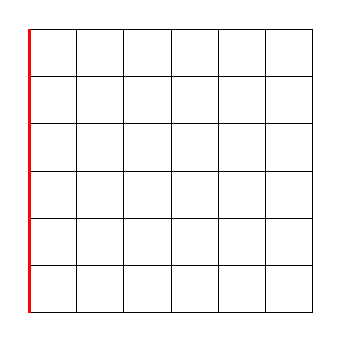
\begin{tikzpicture}[scale=.6]
\draw[step=1] (-3,-3) grid (3,3);
\draw[red, very thick] (-3,-3) -- (-3,3);
\end{tikzpicture}
\end{subfigure}%
\begin{subfigure}{.5\textwidth}
  \caption{$\diff{s}^2 = \diff{r}^2 + r^2\diff{\theta}^2$}
  \centering
    \begin{tikzpicture}
	\pgftransformnonlinear{\circletransformation}
\draw[step=1] (-3,-3) grid (3,3);
\draw[red, very thick] (-3,-3) -- (-3,3);
\end{tikzpicture}
\end{subfigure}
\caption{Transformation $x= r\cos\theta, y= r\sin\theta$}
\end{figure}


\section{Some more geometry}
gravity $\leftrightarrow$ geometry of spacetime

Different (non-Euclidean) geometries possible. Visualization in extra dimension. Also intrinsic definition? 
\begin{itemize}
\item Axiomatic
\item From the distance between nearby points (then larger distances by integration)
\end{itemize}

Any free observer sees the same spacetime, measured with the line element
\[ \diff{s}^2 = \diff{x}^\mu \eta_{\mu\nu}\diff{x}^\nu \]
using the Minkowsky metric. Here we use the mostly plus convention:
\[ \eta = \begin{pmatrix}
-1 & 0 \\
0 & \mathbb{1}_3
\end{pmatrix} \]


\begin{figure}
\centering
\begin{subfigure}{.5\textwidth}
  \centering
    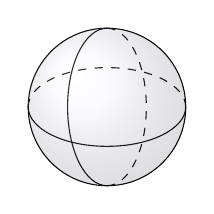
\begin{tikzpicture}
    \draw (-1,0) arc (180:360:1cm and 0.5cm);
    \draw[dashed] (-1,0) arc (180:0:1cm and 0.5cm);
    \draw (0,1) arc (90:270:0.5cm and 1cm);
    \draw[dashed] (0,1) arc (90:-90:0.5cm and 1cm);
    \draw (0,0) circle (1cm);
    \shade[ball color=blue!10!white,opacity=0.20] (0,0) circle (1cm);
\end{tikzpicture}
\end{subfigure}%
\begin{subfigure}{.5\textwidth}
  \centering
    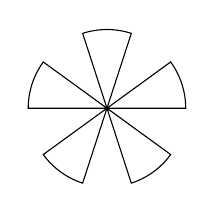
\begin{tikzpicture}
	\foreach \rot in {0,72,...,298} {
\draw[rotate=\rot] (0,0) -- (1cm,0) arc (0:36:1cm) -- (0,0);
}
\end{tikzpicture}
\end{subfigure}
\caption{Positive curvature}
\end{figure}


\begin{figure}
\centering
\begin{subfigure}{.5\textwidth}
  \centering
    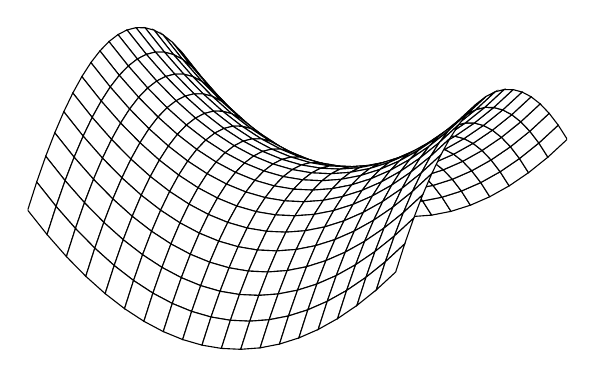
\begin{tikzpicture}
  \begin{axis}[axis lines=none]
    \addplot3[surf, samples=20, color=white, faceted color=black ] {x^2-y^2};
  \end{axis}
\end{tikzpicture}
\end{subfigure}%
\begin{subfigure}{.5\textwidth}
  \centering
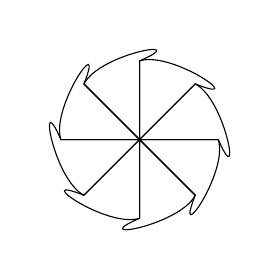
\begin{tikzpicture}
\foreach \rot in {0,45,...,315} {
\draw[rotate=\rot] (0,0) -- (1cm,0) .. controls (1.3cm,-0.7cm) and (1.1cm,.5cm) .. (0.70710678118cm, 0.70710678118cm) -- (0,0);
}
\end{tikzpicture}
\end{subfigure}
\caption{Negative curvature}
\end{figure}

See also intrinsic and extrinsic curvature.
\begin{figure}
\centering
\begin{subfigure}{.5\textwidth}
\caption{Intrinsic curvature}
  \centering
    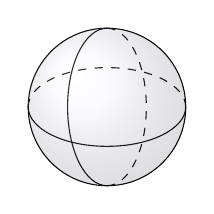
\begin{tikzpicture}
    \draw (-1,0) arc (180:360:1cm and 0.5cm);
    \draw[dashed] (-1,0) arc (180:0:1cm and 0.5cm);
    \draw (0,1) arc (90:270:0.5cm and 1cm);
    \draw[dashed] (0,1) arc (90:-90:0.5cm and 1cm);
    \draw (0,0) circle (1cm);
    \shade[ball color=blue!10!white,opacity=0.20] (0,0) circle (1cm);
\end{tikzpicture}
\end{subfigure}%
\begin{subfigure}{.5\textwidth}
\caption{Extrinsic curvature}
  \centering
    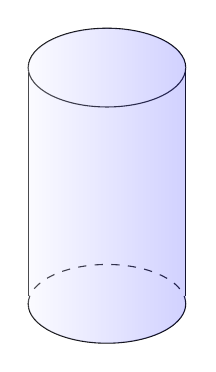
\begin{tikzpicture}
    \draw (-1,0) arc (180:360:1cm and 0.5cm);
    \draw (-1,0) arc (180:0:1cm and 0.5cm);
    \draw (-1,-3) arc (180:370:1cm and 0.5cm);
    \draw[dashed] (-1,-3) arc (180:10:1cm and 0.5cm);
    \draw(-1,-2.9)  -- (-1,0);
    \draw(1,-2.9)   -- (1,0);
    \shade[left color=blue!5!white,right color=blue!60!white,opacity=0.3] (-1,0) arc (180:360:1cm and 0.5cm) -- (1,-3) arc (360:180:1cm and .5cm) -- cycle;
    \shade[left color=blue!5!white,right color=blue!60!white,opacity=0.3] (0,0) circle (1cm and 0.5cm);
\end{tikzpicture}
\end{subfigure}
\caption{Intrinsic and extrinsic curvature}
\end{figure}

\chapter{The equivalence principle}
Given an arbitrary spacetime
\[ \diff{s}^2 = \diff{x}^\mu g_{\mu\nu}(x) \diff{x}^\nu \]
we want the following properties to hold:
\begin{enumerate}
\item Special relativity should be a special case:
\[ g_{\mu\nu}(x) = \eta_{\mu\nu} + \mathcal{O}(x-x_0)^2 \]
\item The same physics should hold for arbitrary transformations
\remark{Coordinates have no meaning}
\item there should be gravity
\end{enumerate}
We have
\[ x^\mu \mapsto x'^\mu = f^\mu(x) \]
with
\[ \diff{x'}^\mu = \Lambda\indices{^\mu_\nu}(x) \diff{x}^\nu \qquad \Lambda \in \GL(1,3) \]
So locally we have a Lorentz group.







